\documentclass[a4paper, 14pt]{extarticle}

\usepackage{../generalPreamble}
\usepackage{../reportFormat}


\begin{document}

\begin{titlepage}
    \centering
    {\bfseries
        \uppercase{
            Минобрнауки России \\
            Санкт-Петербургский государственный \\
            Электротехнический университет \\
            \enquote{ЛЭТИ} им. В.И.Ульянова (Ленина)\\
        }
        Кафедра ИБ

        \vspace{\fill}
        \uppercase{Лабораторная работа №2} \\
        по дисциплине \enquote{Криптография и защита информации} \\
        Тема: Изучение классических шифров Substitution, Permutation/Transposition, Vigenere
    }

    \vspace{\fill}
    \begin{tabularx}{0.8\textwidth}{l X c r}
        Студент гр. 6304 & & \underline{\hspace{3cm}} & Корытов П.В.\\
        Преподаватель & & \underline{\hspace{3cm}} & Племянников А.К.
    \end{tabularx}

    \vspace{1cm}
    Санкт-Петербург \\
    \the\year{}
\end{titlepage}

\newpage

\section*{Цель работы}
Исследовать шифры Substitution, Permutation/Transposition, Vigenere и получить практические навыки работы с ними, в том числе и в программном продукте Cryptool 1 и 2.

\section{Шифр моноалфавитной подстановки}
\subsection{Описание шифра}
Параметры --- Key, Offset
\begin{enumerate}
    \item Первый шаг:
    \begin{itemize}
        \item Удаление всех элементов алфавита, которые присутствуют в кодовом слове
        \item Удвоенные элементы кодового слова слова сливаются в один
    \end{itemize}
    \item Второй шаг
    \begin{itemize}
        \item Задается значение смещение первого элемента кодовго слова (Offset)
        \item По значению смещения определяется количество символов алфавита, полученного после удаления его элементов, которые будут предшествовать вставке когодового слова, после которого запись имеющегося алфавита
    \end{itemize}
\end{enumerate}

\subsection{Формулировка задания}
\begin{enumerate}
    \item Найти шифр в CrypTool 1: Encrypt/Decrypt-> Symmetric (Classic).
    \item Зашифровать и расшифровать текст содержащий только фамилию (транслитерация латиницей) вручную и с помощью шифра c выбранным ключом и смещением Offset≠ 0. Убедиться в совпадении результатов.
    \item Выполнить зашифрование и расшифрование с различными паролями и смещениями Offset и разобраться как формируется алфавит шифрограммы.
    \item Выбрать абзац (примерно 600 символов) из файла English.txt (папка CrypTool / reference) и зашифровать его.
    \item Выполнить атаку на шифротекст, используя приложение из Analysis-> Symmetric Encryption (classic)-> Cipher Text Only.
    \item Повторить шифрование и атаку для тестов примерно в 300 и в 150 символов
    \item Изучите ручное расшифрование для текстов менее 300 символов.
    \item Выбрать новый абзац (примерно 600 символов) из файла English.txt (папка CrypTool/reference) и зашифровать его.
    \item Расшифровать этот абзац, используя приложение Analysis-> Tools for Analysis и Analysis-> Symmetric Encryption (classic)-> Manual Analysis.
    \item  Зашифруйте текст из 200 символов, сохраните ключ, и передайте коллеге для расшифровки.
    \item  Самостоятельно изучите атаки, реализованные CrypTool 2, опираясь на Help и ссылки на статьи.
\end{enumerate}

\subsection{Ход работы}
\begin{enumerate}
    \item Найден шифр в CrypTool 1.
    \begin{figure}[h]
        \centering
        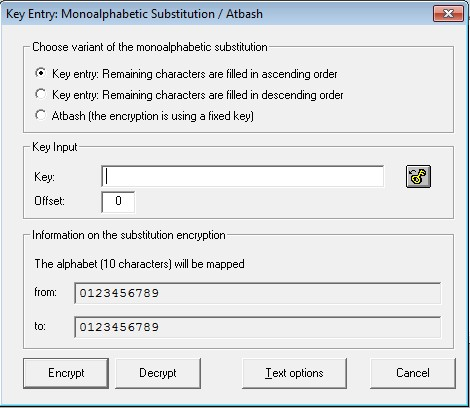
\includegraphics[width=0.7\textwidth]{./img/S001.jpg}
        \caption{Параметры шифра моноалфавитной подстановки в CrypTool 1}
    \end{figure}
    \item Фамилия автора --- KORYTOV, выбранный ключ --- PAVEL.\@ Offset = 5
    \begin{table}[h]
        \centering
        \caption{Таблица шифрования}
        \begin{tabularx}{\textwidth}{@{}XXXXXXXXXXXXX@{}}
        \toprule
        A & B & C & D & E & F & G & H & I & J & K & L & M \\
        B & C & D & F & G & \textbf{P} & \textbf{A} & \textbf{V} & \textbf{E} & \textbf{L} & H & I & J \\ \midrule
        N & O & P & Q & R & S & T & U & V & W & X & Y & Z \\
        K & M & N & O & Q & R & S & T & U & W & X & Y & Z \\ \bottomrule
        \end{tabularx}
    \end{table}
    \begin{itemize}
        \item Результат шифрования фамилии: HMQYSMU
        \item Результат расшифрования: KORYTOV\\
    \end{itemize}
    Результаты совпадают.
    \item Offset сдвигает позицию Key в полученном алфавите
    \item Выбран абзац из текста и зашифрован
    \begin{figure}[h]
        \centering
        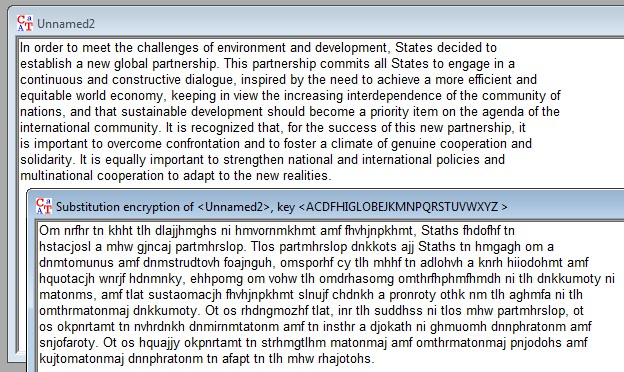
\includegraphics[width=0.8\textwidth]{./img/S002.jpg}
        \caption{Шифрование текста подстановкой}
    \end{figure}
    \item Успешно выполнена атака на текст. Результаты на рисунке~\ref{img:1:3}
    \begin{figure}[h]
        \centering
        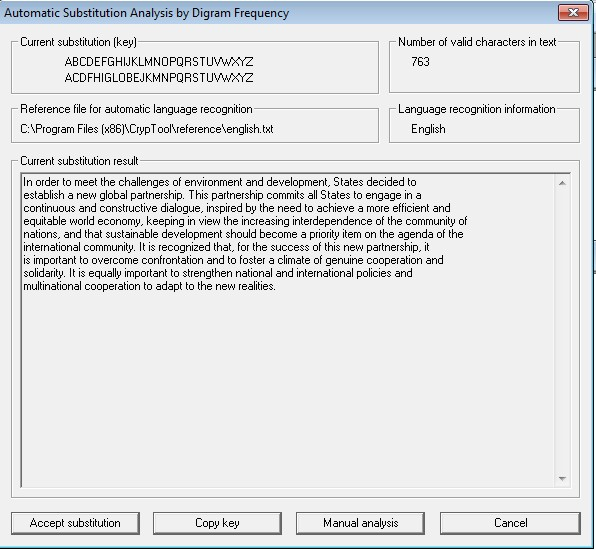
\includegraphics[width=0.8\textwidth]{./img/S003.jpg}
        \caption{Результаты атаки на зашифрованный текст}%
        \label{img:1:3}
    \end{figure}
    \item Выполнены атаки на более короткие тексты:
    \begin{itemize}
        \item Для текста длиной в 300 символов неправильно определена одна буква
        \item Для текста длиной 150 символов около трети букв определено неверно
    \end{itemize}
    \item Ручное расшифрование текста длиной менее 300 символов возможно с помощью частотного анализа и знания слов языка, но является непростой задачей. Подробности в пункте 9.
    \item Зашифрован новый абзац текста
    \item Проведена ручная расшифровка:
    \begin{itemize}
        \item Определена точка расхождения гистограмм частоты букв оригинала и шифротекста. Это смещение --- 3. Буква ключа --- ``D''
        \item С другой стороны алфавита расхождение начинается с ``U'', значит, это часть ключа
        \item После этого поиском корелляций между диаграммами можно установитьещё 
        \item После того, как известна большая часть букв, расшифровка оставшихся --- простая задача, т.к. слова становсятся различимы.
    \end{itemize}
    \item Коллеге зашифрована следующая циатата Ричарда Докинза из книги ``Delusion God'': \\
    ``There is something infantile in the presumption that somebody else (parents in the case of children, God in the case of adults) has a responsibility to give your life meaning and point
Richard Dawkins''\\
    Ключ --- ``ATHEISM'', смещение --- 13
    \item От коллеги получена следующая шифровка:\\
    ``Wf fxnudjrf yns, fvfuy joasuf rajujq fvfuy rbqbpjd anwfu, fvfuy jpdsurjnp ng qif jpgfupbm bevfurbuy, fvfuy mfhjnp fvfuy dnphufhbqjnp bpe ejbcnmjdbm rfdq. Qisr dsurfe efonp bpe fvfuy ejbcnmjdbm mfhjnp wf beksuf yns. Dfbrf qn efdfjvf isobp dufbqsufr bpe qn hjvf qn qifo qif anjrnp ng fqfupbm Afuejqjnp.''
    
    Автоматическая расшифровка дает не очень хороший результат, как видно на рисунке~\ref{img:1:5}
    \begin{figure}[h]
        \centering
        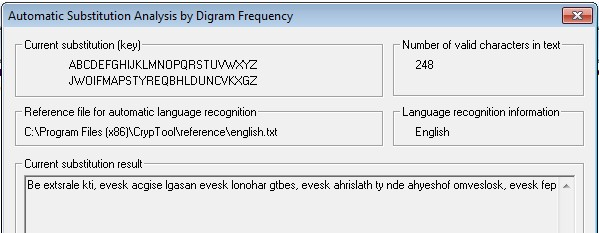
\includegraphics[width=0.7\textwidth]{./img/S005.jpg}
        \caption{Автоматическая расшифровка полученного текста}%
        \label{img:1:5}
    \end{figure}

    С помощью ручной расшифровки удалось восстановить текст. Результаты на рисунке~\ref{img:1:6}
    \begin{figure}[h]
        \centering
        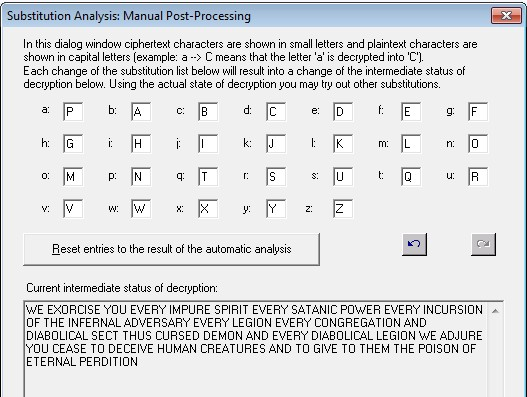
\includegraphics[width=0.7\textwidth]{./img/S006.jpg}
        \caption{Результаты расшифровки}%
        \label{img:1:6}
    \end{figure}

    Как видно, содержание текста --- молитва, изгоняющая демонов. Предположительно, смещение распределения из-за церковных терминов осложнило расшифровку текста.    
    \item В CrypTool 2 реализована атака на шифр путем частотного анализа с восхождением к вершине. Т.е. % TODO

\end{enumerate}

\section{Шифр двойной перестановки (Permutation / Transposition)}
\subsection{Принцип работы шифра}
Текст записывается в матрицу, производится перестановка строк и столбцов

\subsection{Формулировка задания}
\begin{enumerate}
    \item Найти шифр в CrypTool 1: Encrypt/Decrypt-> Symmetric (Classic).
    \item Зашифровать и расшифровать текст, содержащий ФамилиюИмяОтчество (транслитерация латиницей) вручную и с помощью шифра c ключами для перестановки столбцов и строк. Убедиться в совпадении результатов.
    \item Выполнить зашифрование и расшифрование с различными ключами и с различными вариантами перестановки матрицы с текстом по строкам и столбцам. Разобраться с параметрами утилиты.
    \item Зашифровать текст, содержащий ФамилиюИмяОтчество и провести атаку, основанную на знании исходного текста Analysis-> Symmetric Encryption (classic)-> Known Plaintext. 
    \item Зашифровать текст с произвольным сообщением в формате «DEAR messagе THANKS», используя только одинарную перестановку.
    \item Передайте шифровку соседу, для расшифрования при условии, что формы обращения и завершения письма известны.
    \item Самостоятельно изучите атаки, реализованные в CrypTool 2, опираясь на Help и ссылки на статьи.
\end{enumerate}

\subsection{Ход работы}
\begin{enumerate}
    \item Найден шифр в CrypTool 1. Параметры шифра на рисунке~\ref{img:2:1}
    \begin{figure}[h]
        \centering
        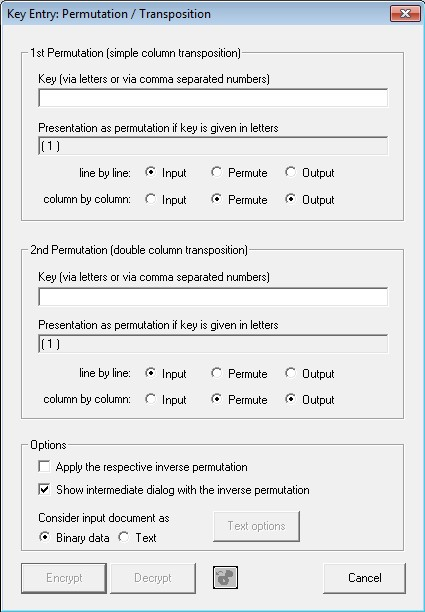
\includegraphics[width=0.6\textwidth]{./img/S007.jpg}
        \caption{Параметры шифра Permutation / Transposition}%
        \label{img:2:1}
    \end{figure}
    \item Текст --- KORYTOVPAVELVALERIEVICH.\@ Ключ --- DACB, DEFBAC.\@ 
    \begin{table}[h]
        \centering
        \begin{tabular}{@{}l|llllll@{}} %chktex 44
         & \textbf{D} & \textbf{A} & \textbf{C} & \textbf{B} \\ \midrule
        \textbf{D} & K & O & R & Y \\
        \textbf{E} & T & O & V & P \\
        \textbf{F} & A & V & E & L \\
        \textbf{B} & V & A & L & E \\
        \textbf{A} & R & I & E & V \\
        \textbf{C} & I & C & H &
        \end{tabular}%
        \hspace{1cm}
        \begin{tabular}{@{}l|llll@{}} % chktex 44
        \textbf{} & \textbf{A} & \textbf{B} & \textbf{C} & \textbf{D} \\ \midrule
        \textbf{D} & O & Y & R & K \\
        \textbf{E} & O & P & V & T \\
        \textbf{F} & V & L & E & A \\
        \textbf{B} & A & E & L & V \\
        \textbf{A} & I & V & E & R \\
        \textbf{C} & C &  & H & I
        \end{tabular}%
        \hspace{1cm}
        \begin{tabular}{@{}l|llllll@{}} % chktex 44
         & \textbf{D} & \textbf{E} & \textbf{F} & \textbf{B} & \textbf{A} & \textbf{C} \\ \midrule
        \textbf{A} & O & O & V & A & I & C \\
        \textbf{B} & Y & P & L & E & V & R \\
        \textbf{C} & V & E & L & E & H & K \\
        \textbf{D} & T & A & V & R & I & 
        \end{tabular}%
        \vspace{0.5cm}
        \begin{tabular}{@{}l|llllll@{}} % chktex 44
         & \textbf{A} & \textbf{B} & \textbf{C} & \textbf{D} & \textbf{E} & \textbf{F} \\ \midrule
        \textbf{A} & I & A & C & O & O & V \\
        \textbf{B} & V & E & R & Y & P & L \\
        \textbf{C} & H & E & K & V & E & L \\
        \textbf{D} & I & R &  & T & A & V
        \end{tabular}
    \end{table}

    Поскольку длина текста --- 23, число операций немного больше. Результат --- IVHIAEERCRKOYVTOPEAVLLV.\@

    CrypTool дает тот же результат --- см. рисунок~\ref{img:2:2}
    \begin{figure}[h]
        \centering
        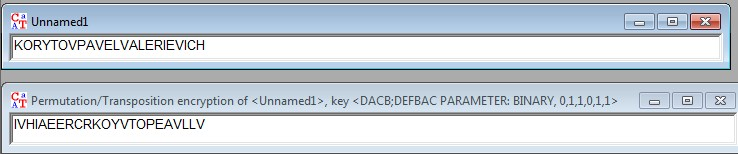
\includegraphics[width=0.9\textwidth]{./img/S008.jpg}
        \caption{Результат CrypTool}%
        \label{img:2:2}
    \end{figure}
    
    Для расшифрования нужно получить обратную перестановку для ключей. Это несложно сделать:
    \begin{table}[h]
        \centering
        \begin{tabular}{@{}llll@{}}
        \toprule
        \textbf{D} & \textbf{A} & \textbf{C} & \textbf{B} \\
        \textit{A} & \textit{B} & \textit{C} & \textit{D} \\ \midrule
        \textbf{A} & \textbf{B} & \textbf{C} & \textbf{D} \\
        \textit{B} & \textit{D} & \textit{C} & \textit{A} \\
        \bottomrule
        \end{tabular}%
        \hspace{2cm}
        \begin{tabular}{@{}llllll@{}}
        \toprule
        \textbf{D} & \textbf{E} & \textbf{F} & \textbf{B} & \textbf{A} & \textbf{C} \\
        \textit{A} & \textit{B} & \textit{C} & \textit{D} & \textit{E} & \textit{F} \\ \midrule
        \textbf{A} & \textbf{B} & \textbf{C} & \textbf{D} & \textbf{E} & \textbf{F} \\
        \textit{E} & \textit{D} & \textit{F} & \textit{A} & \textit{B} & \textit{C} \\
        \bottomrule
        \end{tabular}
    \end{table}
    \FloatBarrier{}
    Обратная перестановка --- BDCA, EDFABC.\@ В столбце с ``C'' будет на один символ меньше, т.к. этот столбец соответствует последнему символу ключа. 
    \begin{table}[h]
        \centering
        \begin{tabular}{@{}l|llllll@{}} % chktex 44
         & \textbf{E} & \textbf{D} & \textbf{F} & \textbf{A} & \textbf{B} & \textbf{C} \\ \midrule
        \textbf{B} & I & A & C & O & O & V \\
        \textbf{D} & V & E & R & Y & P & L \\
        \textbf{C} & H & E & K & V & E & L \\
        \textbf{A} & I & R &  & T & A & V
        \end{tabular}%
        \hspace{2cm}
        \begin{tabular}{@{}l|llllll@{}} % chktex 44
         & \textbf{A} & \textbf{B} & \textbf{C} & \textbf{D} & \textbf{E} & \textbf{F} \\ \midrule
        \textbf{B} & O & O & V & A & I & C \\
        \textbf{D} & Y & P & L & E & V & R \\
        \textbf{C} & V & E & L & E & H & K \\
        \textbf{A} & T & A & V & R & I & 
        \end{tabular}%
    \end{table}

    Теперт пустое место переедет в столбец с ``B'', т.к. это последний символ первой перестановки.
    \begin{table}[h]
        \centering
        \begin{tabular}{@{}l|llll@{}} % chktex 44
        \textbf{} & \textbf{B} & \textbf{D} & \textbf{C} & \textbf{A} \\ \midrule
        \textbf{A} & O & Y & R & K \\
        \textbf{B} & O & P & V & T \\
        \textbf{C} & V & L & E & A \\
        \textbf{D} & A & E & L & V \\
        \textbf{E} & I & V & E & R \\
        \textbf{F} & C &  & H & I
        \end{tabular}%
        \hspace{2cm}
        \begin{tabular}{@{}l|llllll@{}} %chktex 44
         & \textbf{A} & \textbf{B} & \textbf{C} & \textbf{D} \\ \midrule
        \textbf{A} & K & O & R & Y \\
        \textbf{B} & T & O & V & P \\
        \textbf{C} & A & V & E & L \\
        \textbf{D} & V & A & L & E \\
        \textbf{E} & R & I & E & V \\
        \textbf{F} & I & C & H &
        \end{tabular}%
    \end{table}
    
    Расшифрованный текст --- KORYTOVPAVELVALERIEVICH --- совпадает с исходным
\end{enumerate}

\FloatBarrier{}
\section{Шифр Виженера (Vigenere)}
\subsection{Описание шифра}
\begin{itemize}
    \item Заменим буквы алфавита числами соответствующими их порядковым номерам в алфавите $0, 1, \ldots, n-1$.
    \item Представим символы открытого текста $P_i$, ключа $K_i$ и шифротекста $C_i$
    \item Сформируем \dfn{гамму} повторением ключа: $G=(K_1, \ldots, K_M) \ldots (K_1, \ldots, K_m)$
    \item Шифрование символа: $C_i = (P_i + G_i) \bmod n$
    \item Расшифровка символа: $P_i = (C_i - G_i) \bmod n$
\end{itemize}

\subsection{Формулировка задания}
\begin{itemize}
    \item Найти шифр в CrypTool 1: Encrypt/Decrypt-> Symmetric (Classic).
    \item Зашифровать и расшифровать текст, содержащий только фамилию (транслитерация латиницей) вручную и с помощью шифра c выбранным ключом. Убедиться в совпадении результатов.
    \item Произвести атаку на шифротекст, используя приложение Analysis-> Symmetric Encryption (Classic)-> Cipher Text Only->Vigenere.
    \item Повторить атаку для фрагмента текста из файла English.txt (папка CrypTool/reference). Размер текста не менее 1000 символов.
    \item Воспроизведите эту атаку в автоматизированном режиме: 
    \begin{itemize}
        \item Определите размер ключа с помощью приложения Analysis-> Tools for Analysis-> Autocorrelation
        \item Выполните перестановку текста с размером столбца равным размеру ключа приложением Permutation/Transposition
        \item Определите очередную букву ключа приложением Analysis-> Symmetric Encryption (Classic)-> Cipher Text Only->Caesar.
    \end{itemize}
    \item Самостоятельно изучите атаки, реализованные CrypTool 2,
опираясь на Help и ссылки на статьи.
\end{itemize}

\subsection{Ход работы}
\lipsum[1]

\section*{Выводы}

Использованное ПО --- CrypTool 1 / CrypTool 2 в VirtualBox, neovim и \XeLaTeX{} для написания отчета.


\end{document}
